\section{Main matter}

\lipsum[1]

\subsection{Requirements}

\req[req:nolights]{Switch off the lights.}

\req[req:generic_req]{Another requirement.}

\req{A requirement with no label (it can't be referenced in the \LaTeX source)}

\reqlong{A very long requirement (this is only shown in the final table of requirements)}{A very long requirement, possibly including itemized lists:
  \begin{itemize}
  \item Foo;
  \item Bar;
  \item ...
  \end{itemize}}



\subsection{Questions}

\question[q:where]{Where is the coffee machine?}

\question[q:when]{When is the coffee break scheduled?}

\question{A question with no label (it can't be referenced in the \LaTeX source)}

\questionlong{A very long question (this is only shown in the final table of questions)}{A very long question, possibly including enumerated lists:
  \begin{enumerate}
  \item One;
  \item Two;
  \item ...
  \end{enumerate}}







\subsection{Misc. examples}

A quick introduction to \LaTeX{} is available \href{https://www.overleaf.com/learn/latex/Learn_LaTeX_in_30_minutes}{here}.


\subsubsection{Paragraphs}

A single newline will start a new indented paragraph with no vertical space separation.  To add a vertical space you may use \verb|\medskip|, and to avoid indentation you may use \verb|\noindent|. E.g.:

{\it (paragraph starting after a simple newline)} \lipsum[2]

\medskip

{\it (paragraph starting after a \verb|\medskip|)} \lipsum[3]

\medskip

\noindent
{\it (paragraph starting after a \verb|\medskip| and \verb|\noindent|)} \lipsum[4]



\subsubsection{Equations}

\begin{equation}
  \label{eq:eq}
  E = mc^2
\end{equation}


\subsubsection{Lists, footnotes, font types and sizes}

\begin{itemize}
\item {\bf bold};
\item {\it italic};
\item {\tt teletype};
  \begin{itemize}
  \item normal;\footnote{Footnote example.}
  \end{itemize}
\item {\sc Small caps}.
\end{itemize}

\begin{enumerate}
\item {\tiny tiny};
\item {\small small};
\item {\large large};
\item {\Large Large};
  \begin{enumerate}
  \item {\Huge Huge}.
  \end{enumerate}
\end{enumerate}


\subsubsection{Verbatim text}

\begin{verbatim}
Text enclosed inside \texttt{verbatim} environment
is printed in monospace font
and all \LaTeX{} commands are ignored.
\end{verbatim}


\subsection{References}

\begin{itemize}
\item Sect.~\ref{sec:intro}, Sect.~\ref{sec:scope};
\item \citedoc{AD:ESO-123456}, \citedoc{RD:ESO-999999};
\item \citereq{req:nolights}, \citereq{req:generic_req};
\item \citequestion{q:where}, \citequestion{q:when};
\item Tab.~\ref{tab:test}, Fig.~\ref{fig:m31}, Eq.~\ref{eq:eq};
\end{itemize}


\subsection{Figures and tables}

\begin{figure}[hbtp!]
  \centering
  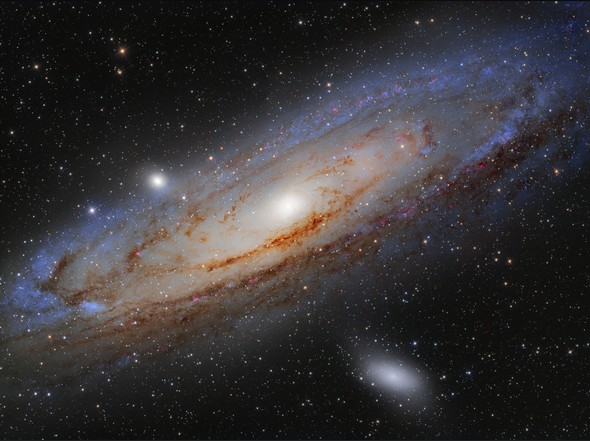
\includegraphics[width=0.5\textwidth]{media/m31}
  \caption{Andromeda galaxy}
    \label{fig:m31}
\end{figure}


\begin{table}[hbtp!]
  \centering
  \caption{Table to test captions and labels.}
  \begin{tabularx}{\textwidth}{|X|X|X|}
    \hline
    \rowcolor{lightgray} \multicolumn{3}{|c|}{Country List} \\
    \hline
    Country Name or Area Name& ISO ALPHA 2 Code &ISO ALPHA 3 \\
    \hline
    Afghanistan & AF &AFG \\
    \rowcolor{gray}
    Aland Islands & AX & ALA \\
    Albania   &AL & ALB \\
    Algeria  &DZ & DZA \\
    American Samoa & AS & ASM \\
    Andorra & AD & \cellcolor[HTML]{AA0044} AND    \\
    Angola & AO & AGO \\
    \hline
  \end{tabularx}
  \label{tab:test}
\end{table}
